\documentclass[useAMS,usenatbib]{mn2e}
\usepackage{footnote,graphicx,natbib,color,multirow,amsmath,url,amssymb,tabularx,hyperref,amssymb, mathtools, listings, float}
\usepackage{aas_macros}
\usepackage[export]{adjustbox}

\hypersetup{
    colorlinks,
    citecolor=blue,
    filecolor=black,
    linkcolor=black,
    urlcolor=black
}

\def\lesssim{\mathrel{\hbox{\rlap{\hbox{\lower3pt\hbox{$\sim$}}}\hbox{\raise2pt\hbox{$<$}}}}}


\begin{document}

\title[AGN feedback in MaNGA]{SDSS-IV  MaNGA: Spatially Resolved Evidence of AGN Feedback}
\author[Smethurst et al. 2021]{R. ~J. ~Smethurst,$^{1}$ et al.
\\ $^1$ Oxford Astrophysics, Department of Physics, University of Oxford, Denys Wilkinson Building, Keble Road, Oxford, OX1 3RH, UK
}

\maketitle

\begin{abstract}
\end{abstract}

\begin{keywords}
galaxies -- photometry, galaxies -- statistics, galaxies -- morphology
\end{keywords}

\section{Introduction}\label{sec:intro}
One of the biggest challenges to $\Lambda$-CDM is the persistent lack of statistically supported evidence of negative AGN feedback occurring across the galaxy population. There are strong theoretical predictions for AGN feedback occurring across the entire galaxy population \citep{Fabian12, Gaibler12}. For example, without AGN feedback to regulate star formation, simulated galaxies grow to unrealistic stellar masses \citep[e.g.][]{silk12}. However, direct observational evidence for quenching caused by AGN across the galaxy population has been elusive. This is in part due to the fact that multiple quenching mechanisms can have similar effects on the observable properties of a galaxy. 

\citet{smethurst16} used optical and NUV global colours to infer the star formation histories of $1,244$ Type 2 AGN. They found that the majority of the AGN had undergone a recent, rapid decline in star formation, not detected in a mass matched control sample of inactive galaxies. This result was promising, suggesting that AGN feedback may be the cause, since AGN have short duty cycles of $\lesssim0.3$~Gyr \citep{martini04} and in simulations are found to cause rapid quenching \citep{tortora09}. However, using the global colours, it was not possible for \citeauthor{smethurst16} to determine whether AGN feedback was the internal cause of the inferred quenching or whether the AGN was merely a consequence of another quenching mechanism (e.g. its activity has been triggered by a galaxy interaction or merger).

 The advent of large IFU galaxy surveys make tackling such a problem possible. In this work we utilise data from the SDSS-IV MaNGA (Mapping Nearby Galaxies at Apache Point Observatory; \citealt{bundy15}) survey, which when complete, will provide a spectrum at 127 individual points (`spaxels') in each of the 10,000 galaxies targeted. Such data allows for spatially resolved quenching histories of galaxies to be determined. This combined with carefully controlling the AGN and control sample selection allows the effects of individual mechanisms, such as AGN feedback, to be isolated.

The overriding expected feature of AGN feedback in derived SFH gradients is that of inside-out quenching, assuming that the feedback proceeds in a quasar-like mode with outflows which progress outward from the galactic centre. However, radio-mode feedback is thought to occur via the heating of the galactic halo which would cut off the global gas supply to a galaxy resulting in a different SFH gradient (this would presumably trace the depletion timescale of the gas, which will be investigated in an upcoming ALMaQUEST paper; Smethurst et al. in prep). 

In this, the first of two papers, we have selected a sample of AGN from the MaNGA MPL-6 sample, along with a magnitude, redshift and IFU size matched control sample. We have derived azimuthally averaged star formation histories for each galaxy using spectral information in conjunction with the SFH inference code \textsc{snitch} \cite{smethurst19a}. In this paper we investigate how the SFHs of AGN compare to the control sample of inactive galaxies, with a second paper (Smethurst et al. 2021b)sinvestgating how the SFHs change with AGN selection method (e.g. optical, X-ray, infrared selected) to investigate the hypothesis that AGN of different types are at different stages in their evolution \cite{hopkinspaper}. 

In Section~\ref{sec:data} we describe the MaNGA data used, and summarise the methods used to select AGN and infer their SFHs. In Section~\ref{sec:results} we present our results along with a discussion in Section~\ref{sec:disc}. Finally, we summarise our findings in Section~\ref{sec:conc}. Where necessary we adopt the Planck 2015 \citep{planck16} cosmological parameters with $(\Omega_m, \Omega_{\lambda}, h) = (0.31, 0.69e, 0.68)$. 

\section{Data \& Methods}\label{sec:data}

\begin{figure*}\label{fig:comparemangacontrol}
\includegraphics[width=0.9\textwidth]{../figures/redshift_gal_abs_rmag_ellison_control_sample.pdf}
\caption{Properties of the AGN sample (black) compared with the matched control sample (red dashed). Shown are the redshift (left) and galaxy absolute u-band magnitude (right; see Section ?). The Anderson-Darling p-values and corresponding $\sigma$ values are also shown in each panel to demonstrate the successful matching of the two samples.}
\end{figure*}

%Figure 2 is an example SDSS cut out with Halpha, Dn4000 maps etc
% this actually needs to be cut out, halpha, dn4000, hbeta, mgfe, hdeltaA - i.e. the ones I actually use in SNITCH
\begin{figure*}\label{fig:mangadap}
\centering{
\includegraphics[width=0.18\textwidth, valign=c]{../figures/8983-12701.png}
\includegraphics[width=0.81\textwidth, valign=c]{../data/ellison/figures/manga_marvin_middle_spectra_8983-12701.png}
\includegraphics[width=0.99\textwidth]{../data/ellison/figures/manga_marvin_spec_indx_maps_8983-12701.png}
\caption{Central spaxel spectrum of MaNGA galaxy ID 8983-12701 (top; with MaNGA IFU hexagonal footprint overlaid on the SDSS cut out shown in the top left) with spectral measurement maps (bottom) showing the spatially resolved equivalent width of the H$\alpha$ emission line, the D$_n4000$ measurement, the H$\beta$ spectral index, the H$\delta_A$ spectral index, and the MgB spectral index as measured by the MaNGA Data Access Pipeline (DAP). Each of these spectral features is used by SNITCH to infer the resolved star formation history. This galaxy is an optical AGN identified using the BPT diagram.}}
\end{figure*}

\begin{figure*}\label{fig:emls}
\centering{
\includegraphics[width=0.99\textwidth]{../data/ellison/figures/emls_idms_radially_binned_AGN_control.png}
\caption{The spatially binned spectral measured by the MaNGA DAP for the \textsc{mangaagn} sample. Each MaNGA AGN is shown by a black line for each spectral feature, from left to right: $\rm{EW}[H\alpha]$, $H\beta$, $MgB$, $H\delta_A$, $D_n4000$. We also show the median value for the \textsc{mangagn} (blue line) and the \textsc{mangacontrol} (red). This figure shows how the star formation sensitive spectral features used to infer the SFHs are on average, very different between the two samples.}}
\end{figure*}

\begin{figure}\label{fig:confidencecheck}
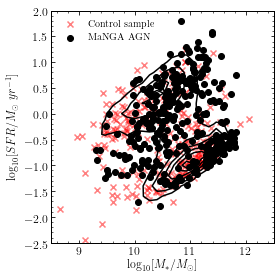
\includegraphics[width=0.45\textwidth]{../data/ellison/figures/manga_agn_SFS_plane.png}
\caption{The stellar mass-star formation rate plane, showing the MaNGA AGN (black circles) and the control sample (red crosses). Also shown in black contours for comparison is the MPA-JHU sample \citep{brinchmann04}, which clearly show the split in the overall galaxy population into the star forming sequence (top left) and quenched population (bottom right).}
\end{figure}


\begin{figure*}\label{fig:agnprop}
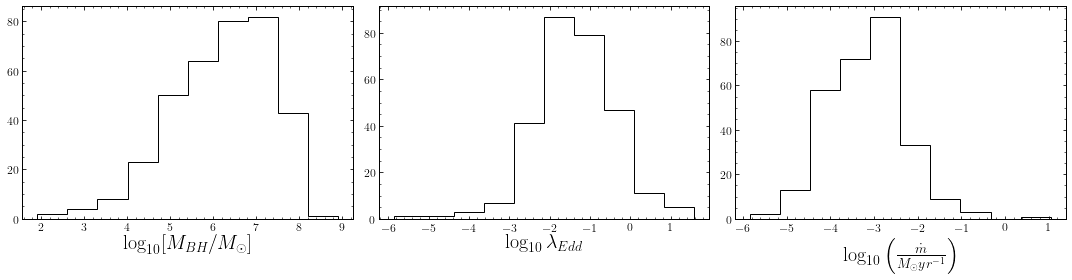
\includegraphics[width=0.9\textwidth]{../data/ellison/figures/mangaagn_sample_agn_properties.png}
\caption{Properties of the MaNGA AGN sample. Shown are the mass of the central supermassive black hole (left; calculated using the method of..., see Section ?), the Eddington ratio (middle) and the accretion rate (right; assuming a radiative efficiency factor $\eta=0.15$, \citealt{elvis02}).}
\end{figure*}

\subsection{MaNGA Data Cubes and Reduction}

MaNGA is a multi-object IFU survey conducted with the $2.5~\rm{m}$ Sloan Foundation $2.5$ meter telescope \citep{gunn06} at Apache Point Observatory (APO) as part of SDSS-IV \citep{blanton17}. By the end of 2021 MaNGA will have observed $\sim10000$ galaxies with $M_* > 10^9~\rm{M}_{\odot}$ \citep[see][for details]{wake17}. 

MaNGA uses the Baryon Oscillation Spectroscopic Survey (BOSS) spectrograph \citep{smee13} which provides continuous coverage between $3600~\AA$ and $10300~\AA$ at a spectral resolution $R \sim 2000$ ($\sigma_{\rm{instrument}} \sim 77 \rm{km}~\rm{s}^{-1}$ for the majority of the wavelength range. 

For the majority of targets, complete spectral coverage to $1.5 R_e$ (effective radius) is obtained (a subset have coverage out to $2.5 R_e$). \cite{bundy15} provides an overview of the MaNGA survey, \cite{drory15} a description of the MaNGA instrumentation, \cite{law15} a description of the observing strategy and \cite{yan16} a description of the survey design. 

The raw MaNGA data was processed by the data reduction pipeline (DRP version 2.0.1), which is discussed in detail in \cite{law16}. The DRP extracts, wavelength calibrates and flux calibrates all spectra obtained in every fibre and exposure. The raw data is then reshaped into a regular gridded datacube of $0.5''$ ‘spaxels’: spatial pixels containing a spectrum at each pixel.  

The MaNGA data analysis pipeline \cite[DAP][]{westfalldap} was developed to fit and analyse the datacubes provided by the DRP The spectral emission lines are masked, and the stellar continuum is modelled using the kinematic and stellar population fitting package \textsc{pxf} \citep{cappellari04}. The stellar continuum model is then constructed using a thinned version of the MILES spectral library (wavelength range $3525 < \lambda~[\rm{\AA}] < 7500$). The model is broadened to match the stellar velocity dispersion of the galaxy in order to cleanly subtract the absorption lines from the spectrum. The residual emission lines are then modelled using Gaussian profiles, with 21 different lines fit in total. The main output from the MaNGA DAP is `maps' of emission lines and absorption featres showing the spatial variation across a galaxy. An example spectra and features maps produced by the DAP are shown for a MaNGA galaxy in Figure~\ref{fig:mangadap}. 

We use the MaNGA DAP to fit both the observed spectrum and synthetic spectrum used in our SFH inference (see Section~\ref{sec:snitch}).

\subsection{AGN Sample Selection}

AGN in MaNGA DR15 were identified by cross-matching (within $5"$) to the sample of AGN from \citet{ellison16}, who identified AGN in the SDSS DR7 main galaxy sample using the BPT diagram \citep[][an optical selection]{bpt}, a cut on WISE colours \citep[$W1 - W2 > 0.8$][an infra-red selection]{wise} and from the LERGs (low excitation radio galaxies) SDSS sample of \citet{heckmanbest12}. We supplement these AGN by also cross matching to the AGN catlogue of \citet{edelson12}, who used ROSAT to identify X-ray luminous AGN. This resulted in a sample consiting of $240$ BPT-selected AGN, $89$ LERGs, $20$ infra-red selected AGN from WISE, and $21$ X-ray selected AGN. A total of $370$ MaNGA AGN. We will refer to this sample as the \textsc{mangaagn} sample. 

We measure the supermassive black hole masses powering these AGN using the method of \cite{who}. From this and the bolometric luminosity we calculate the Eddington ratio and the accretion rate of the black hole. The properties of this sample ($M_{BH}$, $\lambda_{Edd}$ and $\dot{m}$) are shown in Figure~\ref{fig:agnprop}. 

\subsection{Control Sample Selection}

We constructed a control sample of MaNGA galaxies by matching in SDSS $r$-band magnitude, redshift and MaNGA IFU bundle size to the \textsc{mangaagn} sample. This was to control for the galaxy mass and size of each galaxy, and therefore the resulting spatial resolution provided by MaNGA. This resulted in $370$ MaNGA control galaxies which we will refer to as the \textsc{mangacontrol} sample. Figure~\ref{fig:comparemangacontrol} shows the distributions of SDSS $r$-band magnitude and redshift of the \textsc{mangaagn} (black line) and \textsc{mangacontrol} (red line) samples. Anderson-Darling test $p$-values are provided on each panel, and support the hypothesis that the distributions of the two samples are statistically indistinguishable.  

In Figure~\ref{fig:confidencecheck} we also compare the \textsc{mangaagn} (black circles) and \textsc{mangacontrol} (red crosses) on the stellar mass vs. star formation rate plane. Stellar masses and global star formation rates are obtained from the MPA-JHU catalogue \cite{kauffmann03, brinchmann04}. The entire MPA-JHU catalogue is shown by the black contours and represents the overall galaxy population, showing the split into star forming and quenched sequences. The two samples were matched in SDSS $u$-band magnitudes and so have similar stellar mass distributions. The \textsc{mangacontrol} sample have lower star formation rates on average than the AGN sample ($3\sigma$??). Both samples display the bimodal split into star forming and quenched sequences typical of the overall galaxy population.

\subsection{Star Formation Histories with SNITCH}\label{sec:snitch} 

SNITCH is a SFH inference code that was specifically developed for use with MaNGA data \cite[see][for full details, testing and proof of concept]{smethurst19a}, but can be used to quickly infer the analytic SFH of a stellar population from an optical spectrum. The code is open-source \emph{Python} and fully customisable by the user\footnote{https://github.com/rjsmethurst/snitch}. \textsc{SNITCH} uses the Flexible Stellar Population Synthesis models of \cite{conroy09}, the MaNGA Data Analysis Pipeline \cite[DAP][]{mangadap} and a Markov Chain Monte Carlo method \cite[\emph{emcee}][]{emcee13} in order to infer three parameters describing an exponentially declining quenching history: time since quenching, $\Delta t_q$, rate of quenching, $\tau$,  and model metallicity, $Z$. 

For inputs \textsc{snitch} takes emission ($\rm{EW}[H\alpha]$) and absorption ($H\beta$, $H\delta_A$, $MgFe$) spectral features along with $D_n4000$, and their associated errors measured from an observed spectrum. These features were chosen for their sensitivity to either current or past star formation rates, and in the case of $MgFe$ to break the metallicity degeneracy. \textsc{snitch} then assumes values for [$\Delta t_q$, $\tau$, $Z$] to produce a model exponentially declining SFH which is convolved with a stellar population synthesis (SPS) model to generate a synthetic spectrum. Absorption and emission spectral features are then measured in this synthetic spectrum (using the same method used to measure the observed spectrum; in this case the MaNGA DAP) and are then compared to the observed spectral features input. A Bayesian approach is used to determine the likelihood of the assumed SFH model and MCMC is used to infer the best fit SFH for the observed spectrum.
 
The output from \textsc{SNITCH} is therefore a three dimensional MCMC chain charting the [$\Delta t_q$, $\tau$, $Z$] positions explored during the inference (after an initial `burn-in' phase; see \citep{smethurst19a} for details). The ‘best fit’ [$\Delta t_q$, $\tau$, $Z$] values along with their uncertainties can be determined from the 16th, 50th and 84th percentile values of the walker positions.

In order to investigate whether AGN feedback is occurring in the \textsc{mangaagn} sample, we bin the MaNGA data cubes radially and sum the spectra within each radial bin. The number of bins chosen increases with the size of the MaNGA bundle size. For galaxies observed with bundle sizes of [127, 91, 61, 37, 19] fibres, we binned the MaNGA data cubes with [15, 13, 11, 9, 7] logarithmically spaced radial bins respectively (bin numbers chosen through visual inspection). The bin edges were scaled using the effective radius of the observed galaxy using the MaNGA DAP \texttt{proc.spatialbinning.radialbinning} function. Summing the MaNGA `spaxels' in this way is also beneficial as it results in high signal-to-noise ratio (SNR) spectrum in each radial bin, leading to a more accurate measurement of the spectral features. 

Some MaNGA `spaxels' were excluded from the radial bin sum if they were flagged as either starburst or containing broad-line AGN emission (which is not fit by the MaNGA DAP) by a PCA analysis of all of the MaNGA MPL6 `spaxels' \citep{rowlands18}. 

The spectral features for each radial bin were then measured using the MaNGA DAP and input into SNITCH to give best-fit [$\Delta t_q$, $\tau$, $Z$] for each radial bin of a given galaxy, in both the \textsc{mangaagn} and \textsc{mangacontrol} samples.


\section{Results}\label{sec:results}

We first plot the individual radial SFH profiles inferred by SNITCH for all AGN in our sample (black lines), showing the rolling average with radius (blue line) in Figure~\ref{spaghettiall}. We also show the rolling average with radius for the control sample (red). We find that that the average metallicity and time since quenching radial profiles are different in the AGN and the control sample, with AGN quenching more recently than the control sample. The rate of quenching radial profiles are statistically indistinguishable suggesting that the process/processes which quenched the control sample galaxies in the past are responsible for quenching the AGN more recently.

We are most interested in the time since quenching with respect to current AGN activity, therefore we focus on this parameter in the rest of the figures. In Figure~\ref{fig:spaghettimass} we show the time since quenching against radius for the \textsc{mangaagn} sample split into three mass bins (the edges of which were chosen to give equal numbers in each bin). We also show the average value in each radial bin for the control sample in each mass bin (red lines). Lower mass AGN have quenched more recently than high mass AGN, which resemble the control sample. This suggests AGN hosted by high mass galaxies no longer have an impact via AGN feedback, compared to AGN in low mass galaxies. 

In Figure~\ref{fig:spaghettimdot} we split the \textsc{mangaagn} sample by the SMBH accretion rate, $\dot{m}$, once again into three bins of equal numbers. There is very little difference between the radial quenching profiles of low, medium and high accretion rate, suggesting that if AGN feedback is occurring due to outflows from the AGN, then the accretion rate must be independent of the outflow rate.

\begin{figure*}\label{spaghettiall}
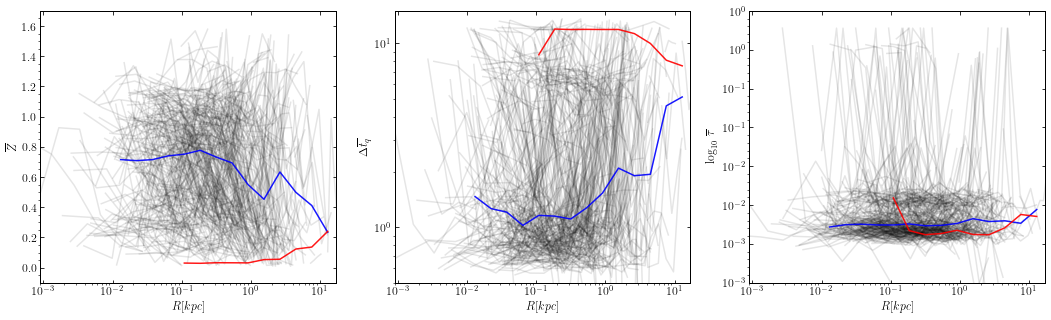
\includegraphics[width=0.9\textwidth]{../data/ellison/figures/manga_agn_spaghetti.png}
\caption{The spatially resolved SFHs with galaxy radius as inferred by \textsc{snitch} for the MaNGA AGN sample. Each MaNGA AGN is shown by a black line for the metallicity (left), time since quenching started (middle) and rate of quenching (right). We also show the median value for bins in the radius for the MaNGA AGN (blue line) and the control sample (red). This figure shows how the quenching histories of current AGN and the control sample are indeed different, in particular, the AGN have quenched more recently than the control sample.}
\end{figure*}

\begin{figure*}
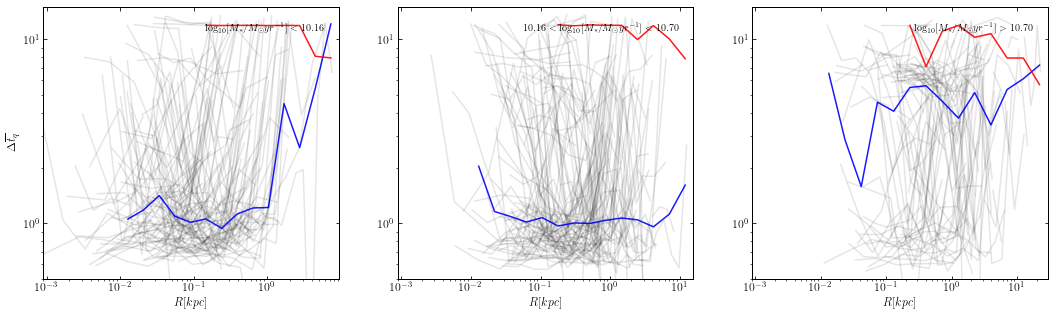
\includegraphics[width=0.9\textwidth]{../data/ellison/figures/median_deltatq_with_kpc_radius_ellison_splitmass.png}
\caption{The spatially resolved time since quenching started against galaxy radius as inferred by \textsc{snitch} for the MaNGA AGN sample, split into low (left), medium (middle) and high (right) stellar mass. These boundaries were chosen to give an equal number of MaNGA AGN in each of the three stellar mass bins. Each MaNGA AGN is shown by a black line. We also show the median value for bins in the radius for the MaNGA AGN (blue line) and the control sample (red) split by stellar mass. This figure shows how lower mass AGN have quenched more recently than high mass AGN, perhaps suggesting that AGN in high mass galaxies have less affect on their host galaxy, supporting results from Smethurst et al. (2016).}
\label{fig:spaghettimass}
\end{figure*}

\begin{figure*}
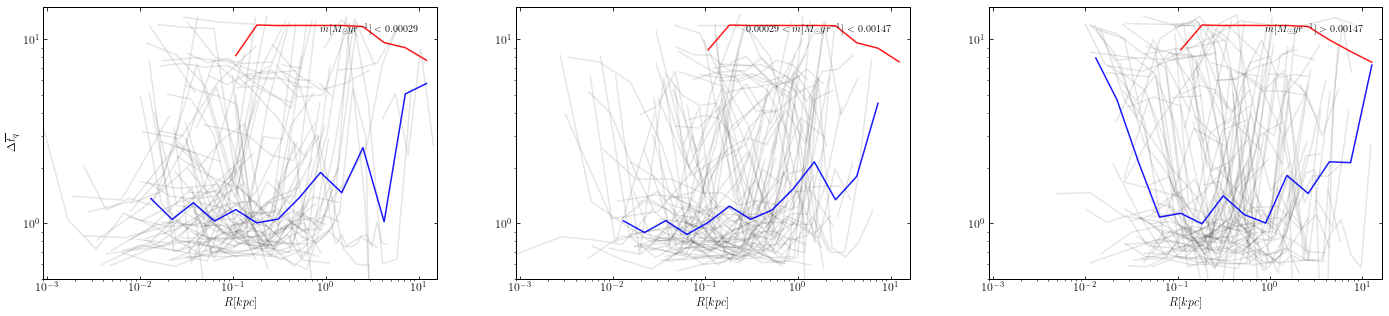
\includegraphics[width=0.9\textwidth]{../data/ellison/figures/median_deltatq_with_kpc_radius_ellison_splitmdot.png}
\caption{The spatially resolved time since quenching started against galaxy radius as inferred by \textsc{snitch} for the MaNGA AGN sample, split into low (left), medium (middle) and high (right) black hole accretion rate. These boundaries were chosen to give an equal number of MaNGA AGN in each of the three accretion rate bins. Each MaNGA AGN is shown by a black line. We also show the median value for bins in the radius for the MaNGA AGN (blue line) and the entire control sample (red). This figure shows how higher accretion rate AGN may have had more effect on their host galaxies in the past.}
\label{fig:spaghettimdot}
\end{figure*}


\section{Discussion}\label{sec:disc}

\section{Conclusions}\label{sec:conc}

\bibliographystyle{mn2e}
\bibliography{refs}  

\end{document}
